\section{TODO: Possible Approaches} % (fold)
\label{sec:possible_approaches}
	This section will describe how the technologies introduced in section \ref{sec:useful_technologies} can be used in combination to form approaches that facilitate server-client portability and facilitate moving JavaScript errors from client to server side. Figure \ref{approachMap} shows a map of the considered approaches, and the rest of this section will briefly explain each of them including their individual benefits and disadvantages. 

	\begin{figure}[H]
		\begin{center}
			\centerline{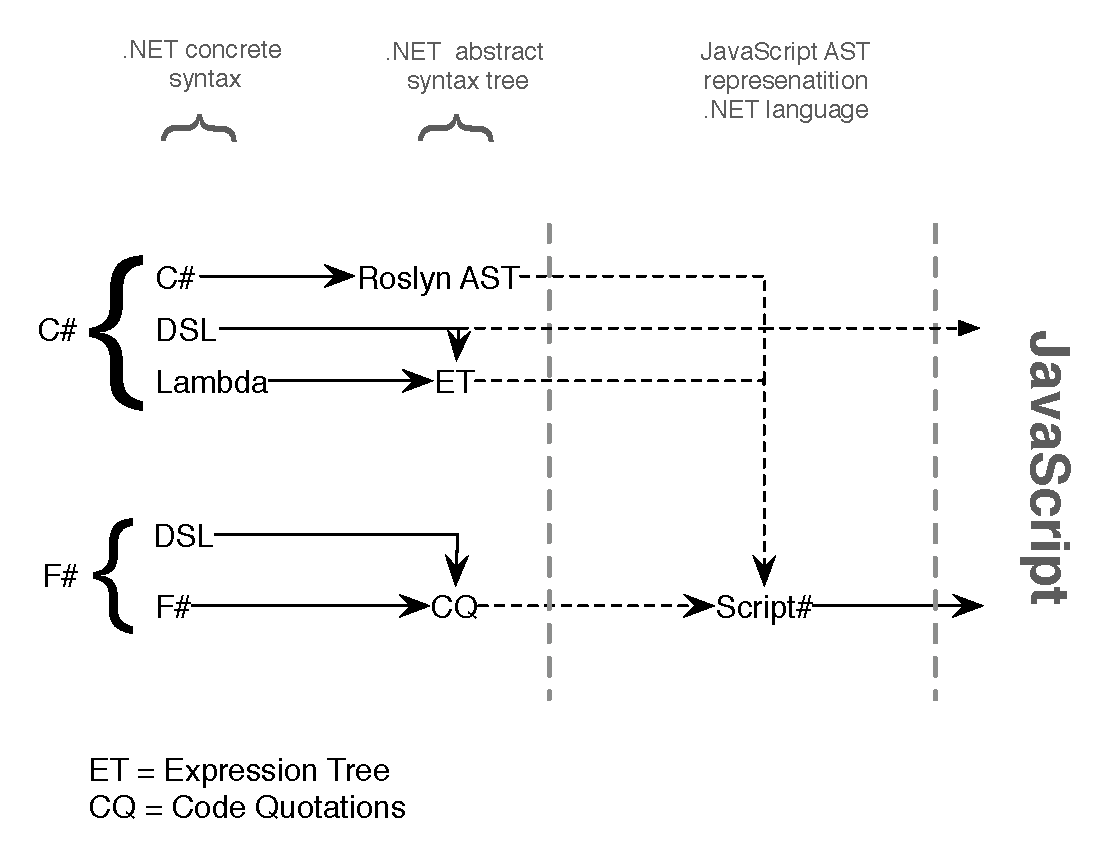
\includegraphics[width=14cm]{resources/images/approachComparison.eps}}
		\end{center}
		\caption{Map of possible approaches. A solid line means that the transition from A to B is given and requires no work on our side. A dashed line means that the transition has to be implemented. Note that the four stages shown in figure \ref{stages} are also reflected in this figure.}
		\label{approachMap}
	\end{figure}

		
	\subsection{C\# to Roslyn to Script\# to JavaScript} % (fold)
	\label{ssub:c_to_roslyn_to_script_to_javascript}
		By using a combination of Roslyn and Script\# it would be possible to first generate an AST representing the developers C\# code. The work on our hand in this solution is then to map the generated C\# AST to a corresponding Script\# AST representing JavaScript. Script\# would then be able to generate JavaScript from this AST.
	% subsection c_to_roslyn_to_script_to_javascript (end)

	\subsection{C\# Internal DSL to JavaScript} % (fold)
	\label{ssub:c_internal_dsl_to_javascript}
		To approach the project initially we did some experiments with a C\# internal DSL from which JavaScript was created directly (i.e. the C\# or F\# abstract syntax tree and JavaScript AST stages are skipped). Using factory methods, operator overloading and a mechanism to handle block scope we arrived at a DSL syntax that could only be somewhat compared to JavaScript concrete syntax. However, the syntax was a bit verbose which decreased readability. 

		Another problem with the C\# DSL implementation was that the assignment operator in C\# could not be overloaded which resulted in inconsistent ways of assigning values to variables. This was a critical problem because wrong use of the '\texttt{=}' operator could cause very subtle errors.

	% subsection c_internal_dsl_to_javascript (end)

	\subsection{C\# Internal DSL to Expression Trees to JavaScript} % (fold)
	\label{ssub:c_internal_dsl_to_expression_trees_to_javascript}

		We considered a variation of the C\# DSL approach which included the use of Expression Trees. This DSL would build an AST consisting of Expression Trees from which JavaScript could be generated (i.e. the C\# or F\# abstract syntax tree stage would be included). This approach would somewhat accommodate Server-Client Portability because Expression Trees can be dynamically compiled and executed as server side code. However this approach inherits the same problems as the C\# DSL approach.
	% subsection c#_internal_dsl_to_expression_trees_to_javascript (end)

	\subsection{C\# Lambda to Expression Trees to Script\# to JavaScript} % (fold)
	\label{ssub:c_lambda_to_expression_trees_to_script_to_javascript}
		Instead of building Expression Trees manually as in the previous DSL approach this approach uses the possibility to generate Expression Trees from lambda expressions. Using lambda expressions would imply that C\# concrete syntax could be used and not a DSL. Therefore the DSL related problems discussed previously, would be avoided which makes this approach superior to the DSL approaches. However an Expression Tree cannot be generated from lambda \emph{statements}. This implies that the use of statements would not be possible with this approach. The use of statements is important writing JavaScript code so this was a critical shortcoming for this approach.
	% subsection c_lambda_to_expression_trees_to_script#_to_javascript (end)

	% subsection csharp_approaches (end)
	
		\subsection{F\# Internal DSL to Script\# to JavaScript} % (fold)
		\label{ssub:f_internal_dsl_to_script_to_javascript}
			An alternative to a C\# internal DSL is an F\# internal DSL. The problem with not being able to overload the assignment operator would not be an issue in F\#. It is even possible to implement new operators consisting of one or more characters from a given set, consequently making it possible to implement some special JavaScript operators such as strict equal (===). An issue with this solution, is that the F\# syntax is very different from the C-like syntax of JavaScript.
		% subsection f_internal_dsl_to_script_to_javascript (end)

		\subsection{F\# Code Quotations to Script\# to JavaScript} % (fold)
		\label{ssub:f_code_quotations_to_script_to_javascript}
			An alternative to using C\# and Roslyn is F\# and Code Quotations. As with Roslyn, the work on our hand would be to map the F\# AST to it's corresponding Script\# JavaScript AST. A disadvantage of using Code Quotations is that they require the developer to know a different language from the one in which ASP.NET Web Forms applications are typically written (C\#). This would probably not be a very great barrier if the syntax of the language didn't vary as much as F\# does from C\#. Also, C\# and JavaScript are somewhat similar in syntax, whereas F\#'s and JavaScripts syntaxes are beyond comparison. A problem related to F\#'s syntax is that the mapping between the F\# AST and the Script\# JavaScript AST could possibly be more difficult than with C\# and Roslyn.
		% subsection f_code_quotations_to_script_to_javascript (end)

	% subsection f_approaches (end)